\documentclass[11pt, a4paper]{article}
\usepackage[a4paper, margin=2.5cm]{geometry}
\usepackage{enumitem}
\setlist[itemize]{label=-}
\usepackage{hyperref}
\usepackage{graphicx}

\title{Analise e Discussao sobre Fluxos Orfaos na Monitorizacao de Redes IP}
\author{[O Teu Nome / Numero de Aluno]}
\date{Outubro de 2026}

\begin{document}

\maketitle

\begin{abstract}
Este ensaio exploratorio, desenvolvido no ambito da avaliacao de Qualidade de Servico em Redes IP (QoSI), apresenta uma analise detalhada do artigo "Understanding Orphan Flows", de Kevin Sam Tharayil et al., direcionado a conferencia TMA (Network Traffic Measurement and Analysis Conference). O trabalho foca-se na problematica dos fluxos de rede sem resolucao DNS associada, explorando os desafios que estes representam para a visibilidade dos operadores de rede, o seu impacto direto na gestao de recursos (QoS) e as vulnerabilidades de seguranca inerentes a evasao de controlos baseados em DNS.
\end{abstract}

\section{Introducao}
A gestao eficaz da Qualidade de Servico (QoS) e a monitorizacao de seguranca em redes IP modernas dependem fortemente de uma visibilidade abrangente sobre o trafego. Tradicionalmente, os administradores de rede utilizam a correlacao entre registos NetFlow (que resumem metadados de comunicacao entre enderecos IP) e dados do Domain Name System (DNS) para identificar e categorizar as aplicacoes em uso.

Contudo, esta abordagem baseada em DNS possui um "ponto cego" significativo: o trafego direcionado a enderecos IP que nao possuem qualquer registo DNS associado. A estes fluxos da-se o nome de fluxos orfaos (orphan flows). Este fenomeno pode resultar de aplicacoes legitimas (como sincronizacao de relogios ou otimizacoes Peer-to-Peer), utilizacao de servicos de anonimizacao (VPNs) ou atividades maliciosas programadas para evadir mecanismos de bloqueio de dominios.

Este trabalho efetua o estudo e analise do artigo atual "Understanding Orphan Flows", extraindo as suas principais conclusoes e discutindo o seu impacto para as tematicas de QoSI, visando preparar uma exposicao critica sobre os desafios contemporaneos da analise de trafego.

\section{Resumo do Artigo: "Understanding Orphan Flows"}

A monitorização do tráfego DNS é um pilar fundamental da gestão e segurança de redes IP modernas. No entanto, este artigo demonstra a existência de um ponto cego crítico: os "Fluxos Órfãos" (Orphan Flows), isto é, comunicações IP direcionadas a endereços que não possuem qualquer pedido DNS prévio registado. O estudo analisa mais de 3.3 mil milhões de registos NetFlow diários, isolando tráfego legítimo omitido bem como vetores de evasão de segurança e malware.

\subsection{Metodologia e Desafios Praticos}
A identificacao de fluxos orfaos a esta escala apresenta enormes desafios operacionais (tipicos na area coberta pela conferencia TMA), nomeadamente a perda de dados na recolha (que no estudo chegou a rondar os 62 por cento na captura de pacotes) e a dificuldade em orientar fluxos unidirecionais. 

Para resolver este problema, os autores construiram um pipeline de processamento de trafego que filtra ruido esperado (como trafego ICMP ou DNS interno), funde fluxos unidirecionais em bidirecionais baseando-se em portas efemeras vs. registadas para inferir a direcao cliente-servidor, e cruza os dados limpos com bases de dados DNS ativas e passivas.

\begin{figure}[htbp]
  \centering
  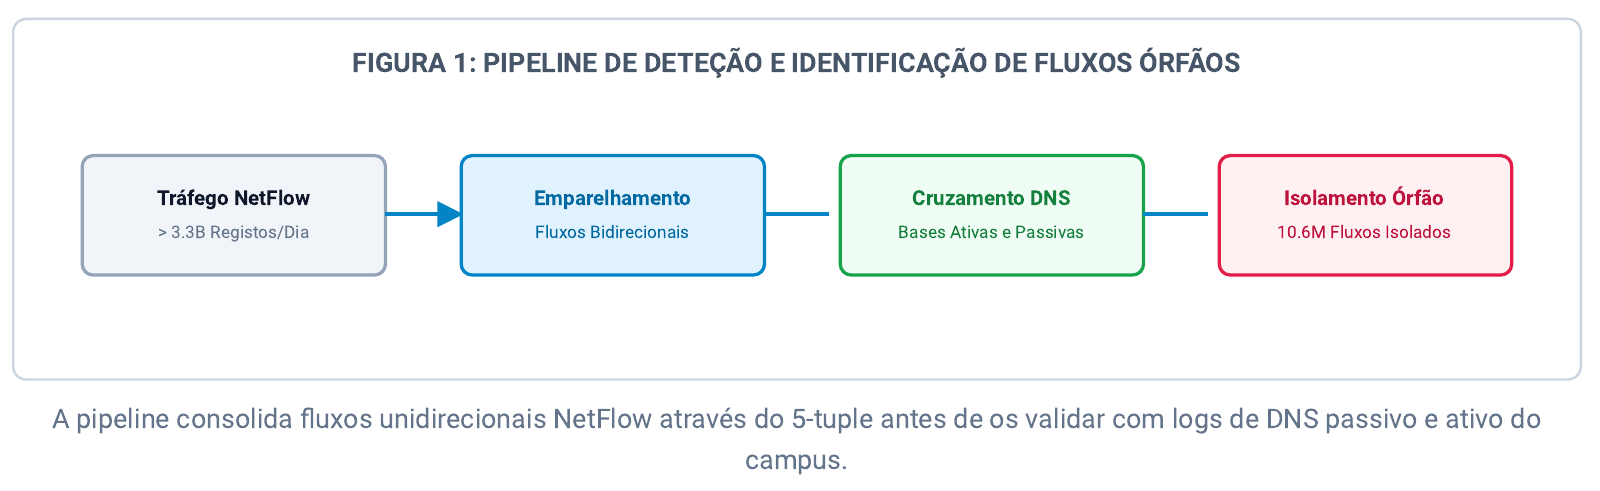
\includegraphics[width=0.8\textwidth]{2.png}
  \caption{Pipeline de deteção e identificação de fluxos órfãos.}
  \label{fig:1}
\end{figure}

\subsection{Principais Descobertas e Classificacao}
Do processamento restaram cerca de 26 mil enderecos IP orfaos, que foram alvo de categorizacao rigorosa:
\begin{itemize}
    \item \textbf{Trafego Explicavel (53,47\%):} Mais de metade dos IPs orfaos pertenciam a comportamentos de rede esperados mas evasivos ao DNS, tais como ligacoes VPN, sistemas de partilha Peer-to-Peer (ex: BitTorrent), atualizacoes otimizadas do Windows e comunicacoes de audio/video via Microsoft Teams.
    \item \textbf{Trafego Malicioso Confirmado (7,27\%):} Correspondente a IPs presentes em listas de bloqueio publicas (blocklists) ou fortemente sinalizados por fornecedores de antivirus.
    \item \textbf{Potencialmente Malicioso (2,53\%):} Enderecos que escapam as atuais listas de bloqueio, mas com os quais ficheiros de malware conhecidos tentaram ativamente comunicar de forma direta por IP.
    \item \textbf{Comportamento Indeterminado (36,73\%):} Destaca a dificuldade intrinseca da medicao de redes reais (wild west da internet), onde uma porcao significativa de trafego permanece incompreensivel apenas por metadados de fluxos.
\end{itemize}

\begin{figure}[htbp]
  \centering
  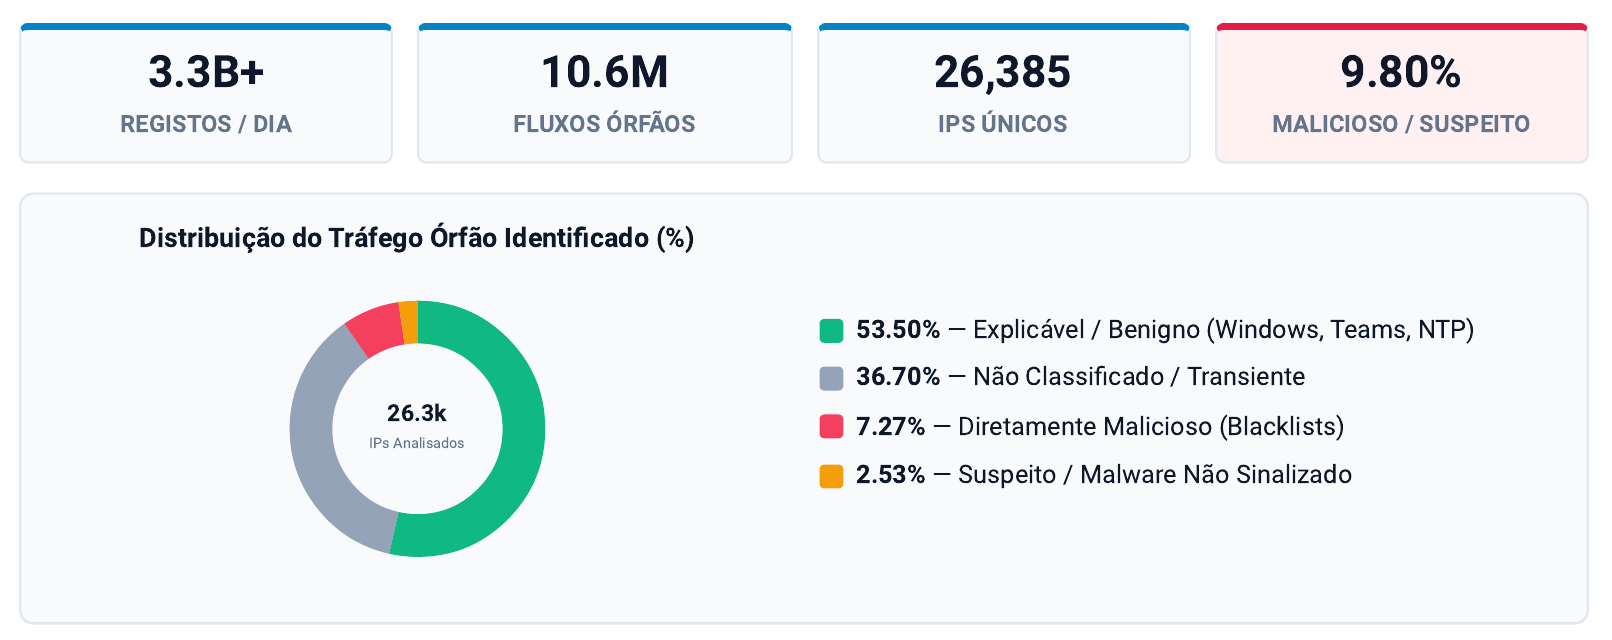
\includegraphics[width=0.8\textwidth]{1.png}
  \caption{Distribuição do Tráfego Órfão Identificado.}
  \label{fig:2}
\end{figure}

O estudo revelou ainda que a esmagadora maioria destes fluxos, em especial os maliciosos, sao altamente transientes, operando ativamente em curtos espacos de tempo e alternando de IP para dificultar a sua detecao.

\section{Discussao e Implicacoes para QoSI}

A introducao do conceito de fluxos orfaos traz implicacoes diretas e profundas para as materias discutidas na unidade curricular de QoSI, estruturando-se em tres grandes eixos de discussao para apresentacao em aula:

\textbf{1. Impacto na Atribuicao de QoS e Gestao de Recursos:} A incapacidade de rotular uma fracao do trafego impede a aplicacao de politicas granulares de QoS. Por exemplo, grandes transferencias de dados via BitTorrent ou atualizacoes Peer-to-Peer do Windows (que geram elevado trafego orfao) podem congestionar a rede e degradar servicos de tempo real. Sem a identificacao DNS, e dificil para os shapers de trafego discernir entre um download secundario e um servico crucial em IP direto.

\textbf{2. O Dilema do "Default Deny" em Redes Fechadas:} Uma reacao intuitiva de seguranca perante fluxos nao identificados seria o seu bloqueio por defeito (default deny). Contudo, a discussao do artigo prova que esta acao causaria quebras de disponibilidade inaceitaveis, uma vez que servicos base como videochamadas, atualizacoes do sistema operativo e sincronizacao NTP (Network Time Protocol) dependem destas conexoes "orfaos". O equilibrio entre seguranca restritiva e usabilidade da rede e um desafio central.

\textbf{3. A Evasao das Defesas Baseadas em DNS:} Grande parte da filtragem e mitigacao de anomalias contemporanea e feita ao nivel do DNS (como firewalls de proxima geracao a bloquear dominios de botnets). A constatacao de que varias familias de malware comunicam exclusivamente por IP direto demonstra uma falha na infraestrutura de medicao tradicional. Para garantir uma rede fiavel e segura, as metricas de desempenho e analise (como defendido pela filosofia da conferencia TMA) devem ser combinadas com inteligncia de ameacas dinamica e sistemas baseados em assinaturas de pacotes em vez de confiarem cegamente no DNS.

\section{Conclusao}

O estudo demonstra inequívocamente que a monitorização exclusiva baseada em DNS deixa lacunas graves de visibilidade. Para manter a Qualidade de Serviço e a Segurança em Redes IP, destacam-se três recomendações fundamentais: 

\textbf{1. Integração de NetFlow + DNS:} Os sistemas de monitorização de rede devem integrar ativamente logs de tráfego IP com respostas DNS em tempo real para assinalar desvios instantaneamente. 

\textbf{2. Deteção de Ameaças Transientes:} Dado que 9.8% dos IPs órfãos estão associados a atividades maliciosas e têm uma vida média curta (efémera), a inspeção de fluxos órfãos serve como um excelente indicador precoce de infeção (IoC). 

\textbf{3. Políticas de QoS e Otimização:} A identificação de tráfego denso (como atualizações P2P do Windows) permite aplicar políticas adequadas de modelação de tráfego (Traffic Shaping) sem afetar aplicações críticas.

\begin{thebibliography}{9}
\bibitem{tharayil2025}
Tharayil, K.S., Avgetidis, A., Ma, Z., Antonakakis, M., Keromytis, A.D.:
\textit{Understanding Orphan Flows}. In: Network Traffic Measurement and Analysis Conference (TMA), 2025.
\end{thebibliography}

\end{document}